\documentclass[11pt,a4paper]{article}

\usepackage[margin=2.5cm]{geometry}
\usepackage{fontspec}
\IfFontExistsTF{Times New Roman}
  {\setmainfont{Times New Roman}}
  {\setmainfont{Liberation Serif}}

\usepackage{amsmath,amssymb}
\usepackage{graphicx}
\usepackage{booktabs}
\usepackage{tabularx}
\usepackage{array}
\usepackage[table]{xcolor}
\usepackage{tikz}
\usetikzlibrary{arrows.meta, positioning, shapes.geometric, calc}
\usepackage{microtype}
\usepackage{csquotes}
\usepackage{enumitem}
\usepackage{setspace}
\usepackage{float}
\usepackage{url}
\usepackage[hidelinks]{hyperref}

\usepackage[backend=biber,style=ext-authoryear,sorting=nyt,maxcitenames=2,mincitenames=1,maxbibnames=99,uniquename=false,uniquelist=false]{biblatex}
\addbibresource{refs.bib}

% Custom color palette
\definecolor{pequiDark}{HTML}{2F4F1F}
\definecolor{pequiGreen}{HTML}{6F8F2F}
\definecolor{pequiLeaf}{HTML}{4F772D}
\definecolor{pequiLight}{HTML}{EEF6D8}
\definecolor{pequiPulp}{HTML}{F2C94C}
\definecolor{pequiPulpLight}{HTML}{FFF4C2}
\definecolor{pequiEarth}{HTML}{A65F2B}
\definecolor{pequiBlue}{HTML}{BFDDE0}
\definecolor{tablehead}{HTML}{EEF6D8}
\definecolor{tablerule}{HTML}{2F4F1F}

\newcolumntype{P}[1]{>{\raggedright\arraybackslash}p{#1}}
\newcolumntype{Y}{>{\raggedright\arraybackslash}X}
\newcolumntype{C}[1]{>{\centering\arraybackslash}p{#1}}

\title{\textbf{Online Constrained Truck Dispatching and Digital Modeling for Agro-Industrial Receiving Yards: A Logistics 5.0 Perspective}}

\author{
  \textbf{Marcus Vinicius Santos da Silva}\textsuperscript{1} \quad
  \textbf{Maria Jos{\'e} Dantas}\textsuperscript{1}\\[0.5em]
  \textsuperscript{1}School of Polytechnic and Arts, Pontifical Catholic University of Goi{\'a}s (PUC Goi{\'a}s),\\
  Goi{\^a}nia, GO, Brazil\\
  \texttt{marcusvinicius@pucgoias.edu.br}, \texttt{mjdantas@pucgoias.edu.br}
}
\date{}

\begin{document}
\maketitle

\begin{abstract}
\noindent\textbf{Paper type:} Original Research Article\\
\textbf{Purpose:} Grain receiving terminals face critical bottlenecks during harvest peaks due to contention for shared resources such as entry gates, scales, and unloading hoppers. Static queue disciplines (e.g., FIFO) fail to react to dynamic operational disruptions such as precipitation over uncovered hoppers, equipment breakdowns, documentation blocks, and contract urgency shifts. This study proposes and evaluates an online constrained dispatching decision-support engine integrated with a 3D digital model, framed within the human-centric and resilience pillars of Logistics 5.0.\\
\textbf{Design/methodology/approach:} Following Design Science Research (DSR), the agro-industrial terminal is modeled as a Dynamic Reentrant Hybrid Flow Shop (RHFS) where entry gross weighing and exit tare weighing share a single physical scale pool. The proposed engine couples multi-stage hard constraint filtering with local short-horizon lexicographic ranking and an auditable event ledger. Computational experiments are conducted using a Discrete-Event Simulation (DES) engine across a 72-cell factorial design with 50 seeds, paired under Common Random Numbers (CRN) against strict FIFO, flow-faithful FIFO, local priority, and fixed-score rules.\\
\textbf{Findings:} Under medium and high congestion strata, the proposed dispatching mechanism achieves a statistically significant reduction ($\ge 15\%$) in the paired 95th percentile (p95) of accumulated queue waiting time without violating protective throughput margins. Concurrently, zero hard constraint violations (A1 safety criterion) and complete structural traceability of decisions and simulated supervisor overrides (A2 governance criterion) are maintained.\\
\textbf{Practical implications:} The artifact provides terminal superintendents and logistics engineers with an explainable, auditable decision-support system that preserves operational safety, accommodates human supervision, and enhances yard resilience under volatile weather and equipment failures.\\
\textbf{Originality/value:} This work addresses the intersection of reentrant hybrid flow shop scheduling, online feasibility filtering, and auditable event logging in bulk agribusiness logistics, establishing an explicit distinction between digital models and digital twins in production engineering.\\
\vspace{0.5em}
\noindent\textbf{Keywords:} online dispatching; agro-industrial yards; discrete-event simulation; digital model; Logistics 5.0; decision support systems.
\end{abstract}

\onehalfspacing

% =========================================================================
\section{Introduction}
\label{sec:introduction}
% =========================================================================

Bulk grain receiving yards in major agricultural producing regions (such as the Brazilian Midwest) represent high-stakes logistics nodes where volatile truck arrival surges collide with rigid infrastructure constraints during harvest seasons \parencite{abdelmagidComprehensiveReviewTruck2022a, graciaTruckAppointmentScheduling2025a}. Road transportation delivers the vast majority of soy, corn, and grains to processing hubs, inland silos, and export ports. When physical handling capacity is strained, long vehicular queues extend onto public highways, triggering severe demurrage penalties, fuel waste, excessive exhaust emissions, and safety hazards \parencite{fioroniFarmPortSimulation2015a, bouyahiaNovelTruckAppointment2025b}.

While static booking and first-in, first-out (FIFO) scheduling paradigms have been widely investigated in maritime container terminals, their direct transposition to agro-industrial receiving yards is hindered by three domain-specific realities:
\begin{enumerate}[leftmargin=1.2cm,itemsep=0pt,topsep=2pt]
  \item \textbf{High operational uncertainty and environmental vulnerability}: Rainfall immediately halts operations at open, uncovered hoppers to protect grain hygroscopic integrity, while mechanical dumper breakdowns and document non-compliances invalidate pre-computed global schedules within minutes \parencite{liProcessSchedulingUncertainty2008a, r.berrutoAnalyzingReceivingOperation2001a}.
  \item \textbf{Reentrant resource contention}: In typical mid-sized terminals, initial gross weighing (laden) and final tare weighing (unladen) share the exact same physical weighbridge installations. Consequently, entry and exit traffic flows actively contend for the same physical servers, creating potential internal deadlocks \parencite{gravesSchedulingReentrantFlow1983, ruizHybridFlowShop2010}.
  \item \textbf{The necessity of human oversight and operational safety}: Automated black-box optimization often fails in practice because terminal operators possess tacit local knowledge and must retain supervisory control. System recommendations must be auditable, explainable, and provably compliant with hard physical and contractual rules \parencite{vanderheydenDecisionSupportSystem1985a, mardanehDecisionSupportSystem2021a}.
\end{enumerate}

These operational realities coincide with the emerging paradigm of \textbf{Logistics 5.0} \parencite{dasilvaIntegrationMachineLearning2023, torbaliMultiagentbasedRealtimeTruck2023}. While Logistics 4.0 focused primarily on hyper-automation, IoT sensors, and efficiency-driven optimization, Logistics 5.0 shifts the emphasis back toward \emph{human-centricity}, \emph{operational resilience}, and \emph{socio-ecological sustainability}. In yard management, this requires systems that empower human dispatchers rather than bypassing them, maintain operational continuity under abrupt disruptions, and traceably guarantee constraint feasibility.

Motivated by these challenges, this study addresses the following research question: \emph{How can an online dispatching decision-support engine be modeled, implemented, and evaluated to dynamically orchestrate truck queues in agro-industrial receiving yards under stochastic disruptions, achieving provable reductions in peak waiting times while guaranteeing zero hard constraint violations and preserving supervisory auditability?}

Adopting the \textbf{Design Science Research (DSR)} methodological framework \parencite{hevnerDesignScienceInformation2004a, peffersDesignScienceResearch2007aa}, we design, formalize, and simulate a computational artifact termed the \emph{PequiFlux Decision Engine}. The core contributions of this paper are fourfold:
\begin{enumerate}[leftmargin=1.2cm,itemsep=0pt,topsep=2pt]
  \item \textbf{Formal Operational Model}: We formulate the grain terminal yard as an online constrained dispatching problem over a \emph{Dynamic Reentrant Hybrid Flow Shop} (RHFS) with shared scale pools and multi-stage precedence.
  \item \textbf{Constrained Lexicographic Dispatching Engine}: We develop a constructive online heuristic combining strict feasibility filtering (removing inadmissible trucks prior to sorting) with local short-horizon lexicographic ranking, eliminating soft penalty tuning and ensuring deterministic execution.
  \item \textbf{Verifiable Safety and Governance Architecture}: We establish dual engineering acceptance criteria: zero hard constraint violations (A1) and an immutable decision ledger supporting full provenance, explainable justifications, and operator override auditability (A2).
  \item \textbf{Decoupled 3D Digital Model}: We architect an event-driven integration between the Discrete-Event Simulation (DES) core and an Unreal Engine~5.8 visualization layer via versioned JSONL logs, strictly adhering to formal international taxonomies distinguishing digital models from digital twins \parencite{kritzingerDigitalTwinManufacturing2018, nistDigitalTwinsEssentialElements2026}.
\end{enumerate}

The remainder of this article is structured as follows. Section~\ref{sec:background} surveys related work on yard management, online scheduling, and Logistics 5.0. Section~\ref{sec:model} formalizes the mathematical problem, hard constraints, and the proposed dispatching algorithm. Section~\ref{sec:protocol} details the factorial experimental design, benchmark policies, and hypothesis testing framework. Section~\ref{sec:results} presents computational results, statistical validations, and managerial implications. Section~\ref{sec:conclusion} concludes with limitations and directions for future research.

% =========================================================================
\section{Theoretical Background and Related Work}
\label{sec:background}
% =========================================================================

\subsection{Yard Management and Truck Scheduling in Bulk Terminals}
Truck scheduling and yard management problems have been intensively studied over the past two decades, with major emphasis on maritime container terminals \parencite{abdelmagidComprehensiveReviewTruck2022a}. Traditional Truck Appointment Systems (TAS) optimize arrival quotas across discrete time windows to flatten arrival peaks \parencite{azabDynamicCollaborativeTruck2017a, bouyahiaNovelTruckAppointment2025b}. However, bulk grain receiving facilities exhibit distinctive physical characteristics that limit the effectiveness of static appointments alone \parencite{t.j.herrmanUseSimulationModel2002a, turnerDiscreteEventSimulation2019a}. 

In grain yards, trucks carry heterogeneous agricultural commodities (e.g., soybeans, corn, sorghum) with varying moisture contents, foreign material percentages, and contractual designations. Once past gate-in inspection, trucks must be routed to specific storage hoppers equipped with compatible mechanical unloading mechanisms (such as hydraulic truck dumpers or drive-over grates) connected to dedicated bucket elevators and silos \parencite{r.berrutoAnalyzingReceivingOperation2001a, m.e.a.inglesEffectsGrainreceivingSystem2006a}. Cross-contamination between non-transgenic and transgenic grain lots is strictly prohibited by industrial quality protocols. Consequently, hopper assignments cannot be treated as uniform parallel servers; they are subject to strict, time-varying routing compatibilities.

\subsection{Dynamic Scheduling and Online Dispatching under Uncertainty}
In production and logistics environments, static offline schedules generated via Mixed-Integer Linear Programming (MILP) rapidly deteriorate when exposed to stochastic disruptions \parencite{liProcessSchedulingUncertainty2008a}. In response, scheduling under uncertainty has evolved along two primary trajectories: proactive (robust or stochastic) programming and reactive/online dispatching \parencite{boysenCrossDockScheduling2010a, nasiriPredictivereactiveCrossdockRescheduling2022}.

In highly dynamic facilities, such as cross-docking terminals and industrial sorting centers, real-time dispatching heuristics that evaluate the system state on a per-event basis provide high computational agility and immediate responsiveness \parencite{langeDispatchingStrategiesDrayage2018a, wangFlexibleStorageYard2023, fonsecaStabilityApproachCDC2025}. Rather than solving large-scale combinatorial models at every state transition, online dispatching applies constructive decision rules upon resource release. Recent studies by \textcite{torbaliMultiagentbasedRealtimeTruck2023} demonstrate that decentralized, rule-based heuristics can achieve operational performance comparable to rolling-horizon mathematical programs while dramatically reducing latency and avoiding numerical non-convergence during high-concurrency peaks.

\subsection{Logistics 5.0 and the Role of Digital Models}
The progression from Industry 4.0 to Industry 5.0—and correspondingly Logistics 5.0—is characterized by a paradigm shift that integrates human ingenuity with smart cyber-physical systems \parencite{dasilvaIntegrationMachineLearning2023}. Whereas earlier automated systems sought to minimize or eliminate human intervention, Logistics 5.0 recognizes that human supervisors remain indispensable for coping with unmodeled edge cases, ethical considerations, and qualitative operational anomalies. Decision support systems in Logistics 5.0 must therefore provide \emph{explainable recommendations} and maintain \emph{transparent governance} \parencite{mardanehDecisionSupportSystem2021a}.

Simultaneously, the widespread deployment of visual representation tools has created conceptual ambiguity regarding digital engineering artifacts. Following the taxonomy established by \textcite{kritzingerDigitalTwinManufacturing2018} and standardized by NIST \parencite{nistDigitalTwinsEssentialElements2026} and ISO \parencite{isoSmartManufacturingWhitePaper2021}:
\begin{itemize}[leftmargin=1.2cm,itemsep=0pt,topsep=2pt]
  \item A \textbf{Digital Model} is a digital representation of a physical system where no automated data flow exists between the physical object and the digital artifact.
  \item A \textbf{Digital Shadow} incorporates a one-way automated data flow from the physical entity to the digital model.
  \item A \textbf{Digital Twin} requires closed-loop, bidirectional, automated real-time data exchange between the physical system and its digital counterpart.
\end{itemize}
In production engineering literature, systems lacking paired real-time telemetric synchronization are frequently mischaracterized as digital twins. In this research, we deliberately classify our Unreal Engine visualizer as a \textbf{Digital Model}, emphasizing its role as an event-driven 3D inspection and replay environment rather than an active telemetry-coupled twin.

% =========================================================================
\section{Problem Formulation and Proposed Dispatching Engine}
\label{sec:model}
% =========================================================================

\subsection{System Description and Physical Layout}
We model an agro-industrial receiving yard comprising four sequential operational stages:
\begin{equation}
  O = \{1, 2, 3, 4\}
\end{equation}
where $o=1$ denotes gate-in document registration and preliminary sampling; $o=2$ denotes initial gross weighing (vehicle plus cargo); $o=3$ denotes grain sampling and unloading at hoppers; and $o=4$ denotes final tare weighing (empty vehicle). 

A critical physical feature of this terminal layout is the \textbf{shared weighbridge pool}. Let $R$ denote the set of all physical resources, and let $B \subset R$ denote the weighbridge pool. Weighbridges $r \in B$ are multi-purpose physical installations serving both gross and tare weighing operations, such that $O(r) = \{2, 4\}$ for all $r \in B$. Gate-in lanes ($o=1$) and unloading hoppers ($o=3$) are dedicated, single-stage facilities. 

This configuration establishes the yard as a \textbf{Dynamic Reentrant Hybrid Flow Shop (RHFS)}:
\begin{itemize}[leftmargin=1.2cm,itemsep=0pt,topsep=2pt]
  \item \emph{Hybrid Flow Shop}: Each stage $o \in O$ possesses multiple parallel physical servers (e.g., $|B| \ge 1$, multiple hoppers).
  \item \emph{Reentrant}: Trucks revisit the exact same resource pool $B$ at stage~4 that they previously occupied at stage~2, creating bidirectional cross-contention between incoming and outgoing traffic.
\end{itemize}

Figures~\ref{fig:yard-layout} and~\ref{fig:flow-diagram} illustrate the terminal layout and the reentrant truck workflow across internal buffer holding zones ($b_1, b_2, b_3$).

% TikZ Figure 1: Yard Layout
\begin{figure}[H]
\centering
\resizebox{0.95\textwidth}{!}{%
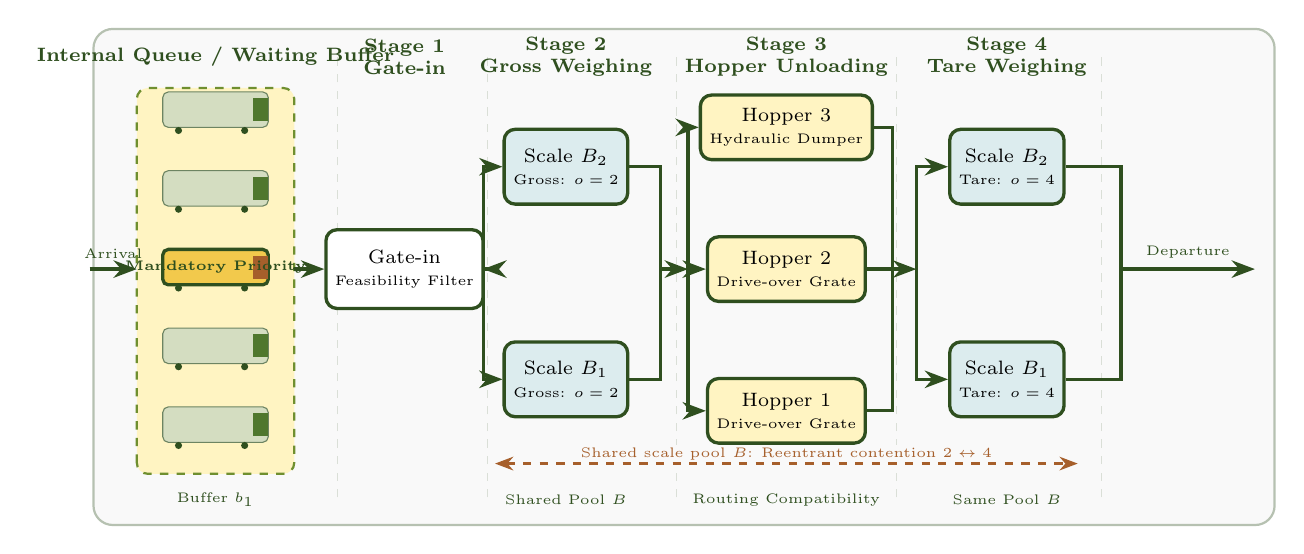
\begin{tikzpicture}[
  >=Stealth,
  font=\scriptsize,
  flow/.style={->, very thick, draw=pequiDark},
  connector/.style={very thick, draw=pequiDark},
  cross/.style={<->, thick, dashed, draw=pequiEarth},
  stagebox/.style={draw=pequiDark, very thick, rounded corners=4pt, align=center},
  label/.style={font=\scriptsize\bfseries, text=pequiDark, align=center}
]
  \fill[gray!5, rounded corners=7pt] (0,0) rectangle (15,6.3);
  \draw[pequiDark!35, thick, rounded corners=7pt] (0,0) rectangle (15,6.3);

  \foreach \x in {3.1,5.0,7.4,10.2,12.8} {
    \draw[pequiDark!18, dashed] (\x,0.35) -- (\x,5.95);
  }

  \node[label] at (1.55,5.95) {Internal Queue / Waiting Buffer};
  \node[label] at (3.95,5.95) {Stage 1\\Gate-in};
  \node[label] at (6.0,5.95) {Stage 2\\Gross Weighing};
  \node[label] at (8.8,5.95) {Stage 3\\Hopper Unloading};
  \node[label] at (11.6,5.95) {Stage 4\\Tare Weighing};

  % Buffer area
  \fill[pequiPulpLight, rounded corners=4pt] (0.55,0.65) rectangle (2.55,5.55);
  \draw[pequiGreen, thick, dashed, rounded corners=4pt] (0.55,0.65) rectangle (2.55,5.55);

  \foreach \y in {1.05,2.05,4.05,5.05} {
    \filldraw[fill=pequiGreen!30, draw=pequiDark!70, rounded corners=2pt] (0.88,\y) rectangle (2.22,\y+0.45);
    \fill[pequiLeaf] (2.02,\y+0.08) rectangle (2.22,\y+0.37);
    \fill[pequiDark] (1.08,\y-0.04) circle (0.045);
    \fill[pequiDark] (1.92,\y-0.04) circle (0.045);
  }
  \filldraw[fill=pequiPulp, draw=pequiDark, very thick, rounded corners=2pt] (0.88,3.05) rectangle (2.22,3.50);
  \fill[pequiEarth] (2.02,3.13) rectangle (2.22,3.42);
  \fill[pequiDark] (1.08,3.01) circle (0.045);
  \fill[pequiDark] (1.92,3.01) circle (0.045);
  \node[font=\tiny\bfseries, text=pequiDark] at (1.55,3.28) {Mandatory Priority};

  \node[stagebox, fill=white, minimum width=1.05cm, minimum height=1.0cm] (gate) at (3.95,3.25)
    {Gate-in\\{\tiny Feasibility Filter}};

  \node[stagebox, fill=pequiBlue!55, minimum width=1.45cm, minimum height=0.95cm] (scaleA) at (6.0,4.55)
    {Scale $B_2$\\{\tiny Gross: $o=2$}};
  \node[stagebox, fill=pequiBlue!55, minimum width=1.45cm, minimum height=0.95cm] (scaleB) at (6.0,1.85)
    {Scale $B_1$\\{\tiny Gross: $o=2$}};

  \node[stagebox, fill=pequiPulpLight, minimum width=1.55cm, minimum height=0.82cm] (hopperA) at (8.8,5.05)
    {Hopper 3\\{\tiny Hydraulic Dumper}};
  \node[stagebox, fill=pequiPulpLight, minimum width=1.55cm, minimum height=0.82cm] (hopperB) at (8.8,3.25)
    {Hopper 2\\{\tiny Drive-over Grate}};
  \node[stagebox, fill=pequiPulpLight, minimum width=1.55cm, minimum height=0.82cm] (hopperC) at (8.8,1.45)
    {Hopper 1\\{\tiny Drive-over Grate}};

  \node[stagebox, fill=pequiBlue!55, minimum width=1.45cm, minimum height=0.95cm] (scaleOutA) at (11.6,4.55)
    {Scale $B_2$\\{\tiny Tare: $o=4$}};
  \node[stagebox, fill=pequiBlue!55, minimum width=1.45cm, minimum height=0.95cm] (scaleOutB) at (11.6,1.85)
    {Scale $B_1$\\{\tiny Tare: $o=4$}};

  \draw[flow] (-0.05,3.25) -- (0.55,3.25) node[midway, above, font=\tiny, text=pequiDark]{Arrival};
  \draw[flow] (2.55,3.25) -- (gate.west);
  \coordinate (afterGate) at (4.95,3.25);
  \coordinate (afterScales) at (7.20,3.25);
  \coordinate (afterHoppers) at (10.15,3.25);
  \coordinate (beforeOutScales) at (10.45,3.25);
  \coordinate (afterOutScales) at (13.05,3.25);

  \draw[flow] (gate.east) -- (afterGate);
  \draw[flow] (afterGate) |- (scaleA.west);
  \draw[flow] (afterGate) |- (scaleB.west);

  \draw[connector] (scaleA.east) -| (afterScales);
  \draw[connector] (scaleB.east) -| (afterScales);
  \draw[flow] (afterScales) -- (7.55,3.25);
  \draw[flow] (7.55,3.25) |- (hopperA.west);
  \draw[flow] (7.55,3.25) -- (hopperB.west);
  \draw[flow] (7.55,3.25) |- (hopperC.west);

  \draw[connector] (hopperA.east) -| (afterHoppers);
  \draw[connector] (hopperB.east) -- (afterHoppers);
  \draw[connector] (hopperC.east) -| (afterHoppers);
  \draw[flow] (afterHoppers) -- (beforeOutScales);
  \draw[flow] (beforeOutScales) |- (scaleOutA.west);
  \draw[flow] (beforeOutScales) |- (scaleOutB.west);

  \draw[connector] (scaleOutA.east) -| (afterOutScales);
  \draw[connector] (scaleOutB.east) -| (afterOutScales);
  \draw[flow] (afterOutScales) -- (14.75,3.25) node[midway, above, font=\tiny, text=pequiDark]{Departure};

  \draw[cross] (5.10,0.78) -- node[above, font=\tiny, text=pequiEarth, fill=gray!5, inner sep=1pt]
    {Shared scale pool $B$: Reentrant contention $2 \leftrightarrow 4$} (12.50,0.78);

  \node[font=\tiny, text=pequiDark] at (1.55,0.32) {Buffer $b_1$};
  \node[font=\tiny, text=pequiDark] at (6.0,0.32) {Shared Pool $B$};
  \node[font=\tiny, text=pequiDark] at (8.8,0.32) {Routing Compatibility};
  \node[font=\tiny, text=pequiDark] at (11.6,0.32) {Same Pool $B$};
\end{tikzpicture}%
}
\caption{Schematic top-down layout of the agro-industrial receiving yard showcasing the four operational stages and the reentrant weighbridge pool.}
\label{fig:yard-layout}
\end{figure}

% TikZ Figure 2: Operational Flow
\begin{figure}[H]
\centering
\resizebox{0.95\textwidth}{!}{%
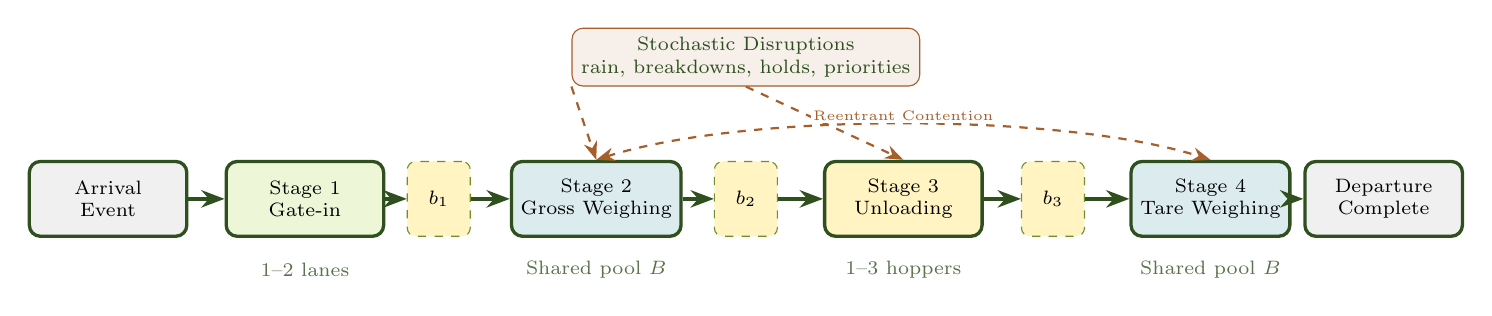
\begin{tikzpicture}[>=Stealth, font=\scriptsize,
    flowstep/.style={draw=pequiDark, very thick, rounded corners=4pt, minimum width=2.0cm, minimum height=0.95cm, align=center},
    buf/.style={draw=pequiGreen, rounded corners=3pt, minimum width=0.8cm, minimum height=0.95cm, align=center, fill=pequiPulpLight, dashed, font=\scriptsize},
    lbl/.style={font=\scriptsize, text=pequiDark!80, align=center},
    flow/.style={->, very thick, draw=pequiDark},
    event/.style={->, dashed, thick, draw=pequiEarth},
    shared/.style={<->, dashed, thick, draw=pequiEarth}]

  \node[flowstep, fill=gray!12]        (arr) at (0,0)    {Arrival\\Event};
  \node[flowstep, fill=pequiLight]     (g1)  at (2.5,0)  {Stage 1\\Gate-in};
  \node[buf]                          (b1)  at (4.2,0)  {$b_1$};
  \node[flowstep, fill=pequiBlue!55]   (w1)  at (6.2,0)  {Stage 2\\Gross Weighing};
  \node[buf]                          (b2)  at (8.1,0)  {$b_2$};
  \node[flowstep, fill=pequiPulpLight] (dsc) at (10.1,0) {Stage 3\\Unloading};
  \node[buf]                          (b3)  at (12.0,0) {$b_3$};
  \node[flowstep, fill=pequiBlue!55]   (w2)  at (14.0,0) {Stage 4\\Tare Weighing};
  \node[flowstep, fill=gray!12]        (out) at (16.2,0) {Departure\\Complete};

  \foreach \a/\b in {arr/g1,g1/b1,b1/w1,w1/b2,b2/dsc,dsc/b3,b3/w2,w2/out} {
    \draw[flow] (\a) -- (\b);
  }

  \node[lbl] at (2.5,-0.9)  {1--2 lanes};
  \node[lbl] at (6.2,-0.9)  {Shared pool $B$};
  \node[lbl] at (10.1,-0.9) {1--3 hoppers};
  \node[lbl] at (14.0,-0.9) {Shared pool $B$};

  \node[draw=pequiEarth, fill=pequiEarth!10, rounded corners=4pt,
        font=\scriptsize, text=pequiDark, align=center, minimum width=3.8cm] (ev) at (8.1,1.8)
        {Stochastic Disruptions\\rain, breakdowns, holds, priorities};
  \draw[event] (ev.south west) -- (w1.north);
  \draw[event] (ev.south) -- (dsc.north);
  \draw[shared] (w1.north) .. controls (8.1,1.1) and (12.1,1.1) ..
    node[above, font=\tiny, text=pequiEarth, fill=white, inner sep=1pt]{Reentrant Contention} (w2.north);
\end{tikzpicture}%
}
\caption{State flow of trucks traversing the yard with intermediate holding buffers and cross-stage reentrant contention.}
\label{fig:flow-diagram}
\end{figure}

\subsection{Discrete-Event System State and Operational Hard Constraints}
Let $k \in \mathbb{R}_{\ge 0}$ denote the continuous simulation clock time. The complete yard state at decision epoch $k$ is defined by the tuple:
\begin{equation}
  S_k = \langle \pi_k, u_k, b_k, d_k, m_k \rangle
\end{equation}
where $\pi_k = \{\pi_{k,o}\}_{o \in O}$ denotes the active truck queues per stage; $u_k = \{u_{k,r}\}_{r \in R}$ registers the next available timestamp for each physical resource $r$; $b_k = \{b_{k,o}\}_{o \in O}$ tracks the buffer occupancy preceding stage $o$; $d_k$ aggregates truck administrative and cargo state attributes; and $m_k$ represents environmental yard conditions (e.g., active precipitation, resource outage flags).

Let $T$ denote the set of trucks, and let $q_i(k) \in O$ denote the next pending operation for truck $i \in T$. When resource $r \in R$ becomes idle at epoch $k$, it can potentially serve trucks from any operation $o \in O(r)$. The set of candidate trucks eligible for resource $r$ is given by:
\begin{equation}
  C_{k,r} = \bigcup_{o \in O(r)} C^{(o)}_{k,r}, \quad C^{(o)}_{k,r} = \left\{\, i \in \pi_{k,o} : q_i(k)=o,\; r \in R_i(o),\; \mathcal{F}_{i,r}(k)=1 \,\right\}
\end{equation}
where $R_i(o) \subseteq R$ is the set of resources capable of performing operation $o$ for truck $i$, and $\mathcal{F}_{i,r}(k) \in \{0, 1\}$ is a strict, conjunctive feasibility indicator:
\begin{equation}
\begin{aligned}
  \mathcal{F}_{i,r}(k) = \mathbb{I}\Big( & \mathrm{Arr}_i \le k \;\land\; \mathrm{CompPrev}_i(k) \;\land\; \mathrm{Cap}_r(k) > 0 \;\land\; \mathrm{PhysComp}_{i,r} \\
  & \land\; \mathrm{DocRel}_i(k) \;\land\; \mathrm{Weather}_{i,r}(k) \;\land\; \mathrm{BufAvail}_{q_i(k)+1}(k) \Big)
\end{aligned}
\end{equation}

In our formulation, feasibility is treated as a \textbf{hard constraint}. Inadmissible candidates are strictly pruned before ranking; unfeasible assignments are never permitted via soft penalty relaxation. The operational constraints enforce:
\begin{enumerate}[leftmargin=1.2cm,itemsep=0pt,topsep=2pt]
  \item \textbf{Arrival and Sequence Precedence}: Truck $i$ must have physically entered the yard ($\mathrm{Arr}_i \le k$) and completed stage $q_i(k)-1$.
  \item \textbf{Physical Resource Compatibility}: Equipment must match truck specifications (e.g., standard tippers require hydraulic dumpers, whereas bottom-discharge hopper trailers require drive-over grates).
  \item \textbf{Administrative and Quality Holds}: Trucks with unverified fiscal documentation or pending laboratory moisture inspection are blocked ($\mathrm{DocRel}_i(k) = 0$).
  \item \textbf{Weather Sensitivity}: Uncovered hoppers cannot accept trucks during active rainfall events ($\mathrm{Weather}_{i,r}(k) = 0$).
  \item \textbf{Buffer Spillover Protection}: A truck cannot begin processing if the downstream intermediate buffer $b_{q_i(k)+1}$ is saturated.
\end{enumerate}

\subsection{Admissibility Domain Construction}
Let $p(i) \in \{0, 1, 2\}$ denote the operational priority of truck $i$, where $p(i)=2$ designates mandatory contractual priority (e.g., pre-scheduled direct export vessel trains or moisture-critical grain). Let $W_i(k)$ represent the time elapsed since truck $i$ became eligible for operation $q_i(k)$, and let $\tau_{p(i)}$ denote the agreed operational tolerance threshold. Operational pressure is defined as:
\begin{equation}
  \mathrm{pressure}_i(k) = \max\left\{ 0,\, W_i(k) - \tau_{p(i)} \right\}
\end{equation}

To prevent myopic sorting over massive queues while guaranteeing immediate responsiveness to critical trucks, the engine builds the \textbf{admissibility domain} $C^{adm}_{k,r}$ via a deterministic two-tier logic:
\begin{equation}
  C^{adm}_{k,r} =
  \begin{cases}
    C^{2}_{k,r} = \{\, i \in C_{k,r} : p(i) = 2 \,\}, & \text{if } C^{2}_{k,r} \neq \emptyset; \\[4pt]
    \mathrm{Top}^{\,\text{arrival}}_{H_0}(C_{k,r}) \;\cup\; \left\{\, i \in C_{k,r} : \mathrm{pressure}_i(k) > 0 \,\right\}, & \text{otherwise.}
  \end{cases}
  \label{eq:cadm}
\end{equation}
Here, $H_0 = 6$ is a frozen short-horizon window that restricts standard sorting to the top-6 arriving feasible trucks, while any truck exceeding its waiting tolerance ($\mathrm{pressure}_i(k) > 0$) is dynamically pulled into the admissible set regardless of its arrival position. Thus, $H_0$ governs ordinary competition, whereas $\tau_p$ governs urgent escalation.

\subsection{Short-Horizon Lexicographic Selection Rule}
When resource $r$ becomes available at epoch $k$, the engine selects the winning candidate $y_{k,r} \in C^{adm}_{k,r}$ using a multi-criteria lexicographic maximization:
\begin{equation}
  y_{k,r} =
  \begin{cases}
    \displaystyle \operatorname*{arg\,lexmax}_{i \in C^{adm}_{k,r}} \; h_{k,r}(i), & \text{if } C^{adm}_{k,r} \neq \emptyset; \\[6pt]
    \emptyset, & \text{otherwise (forced idle; logged with cause).}
  \end{cases}
  \label{eq:lexmax}
\end{equation}
The evaluation vector $h_{k,r}(i)$ is defined as:
\begin{equation}
  h_{k,r}(i) = \left\langle\, \hat{P}_i(k),\; \hat{W}_i(k),\; -\hat{R}_{k,r}(i),\; \hat{A}_{i,r}(k) \,\right\rangle
\end{equation}
where:
\begin{itemize}[leftmargin=1.2cm,itemsep=0pt,topsep=2pt]
  \item $\hat{P}_i(k) = \dfrac{\mathrm{pressure}_i(k)}{\max_{j \in C^{adm}_{k,r}} \mathrm{pressure}_j(k)}$ is the normalized operational urgency pressure;
  \item $\hat{W}_i(k) = \dfrac{W_i(k)}{\max_{j \in C^{adm}_{k,r}} W_j(k)}$ is the normalized waiting duration in the current queue;
  \item $\hat{R}_{k,r}(i) = \dfrac{R_{k,r}(i)}{\max(1, |C^{adm}_{k,r}| - 1)}$ penalizes deviation from strict arrival ordering ($R_{k,r}(i)$ is the number of earlier arrivals bypassed);
  \item $\hat{A}_{i,r}(k) \in \{0, 1\}$ is a setup affinity indicator (1 if hopper $r$ already contains identical grain type, requiring no purge).
\end{itemize}

The lexicographic operator strictly prioritizes criteria hierarchically: pressure $\hat{P}$ strictly dominates waiting time $\hat{W}$, which in turn strictly dominates reordering penalty $\hat{R}$, and finally setup affinity $\hat{A}$. In contrast to weighted linear sums, the lexicographic structure guarantees non-compensatory decision-making, ensuring that contractual commitments and critical delays are never sacrificed for marginal setup gains. The selection runs in $O(|C^{adm}_{k,r}|)$ time, delivering deterministic millisecond-level responsiveness suitable for real-time edge execution.

\subsection{Safety, Explainability, and Supervisory Governance (A1 / A2)}
In alignment with Logistics 5.0, the artifact incorporates two architectural guarantees:
\begin{itemize}[leftmargin=1.2cm,itemsep=0pt,topsep=2pt]
  \item \textbf{Criterion A1 (Operational Safety)}: For every issued dispatch decision $y_{k,r}$, the system computes the post-decision state assertion. A1 requires a zero-tolerance ($0\%$) violation rate across all hard constraints throughout the entire operating horizon.
  \item \textbf{Criterion A2 (Governance and Supervisory Auditability)}: Every decision emits an immutable, cryptographically hashed JSONL record capturing: timestamp $k$, resource $r$, selected candidate $y_{k,r}$, full admissible domain $C^{adm}_{k,r}$, explicit ranking values, and a human-readable textual rationale. If a human terminal supervisor overrides the automated recommendation ($y_{k,r} \leftarrow \text{override}$), the engine verifies the proposed override against hard constraints; if feasible, it executes the override, logging the operator identifier and justification.
\end{itemize}

% =========================================================================
\section{Experimental Design and Evaluation Protocol}
\label{sec:protocol}
% =========================================================================

\subsection{Full Factorial Design Matrix}
The performance of the proposed engine is evaluated using a full factorial experimental matrix implemented in a custom Discrete-Event Simulation (DES) testbed written in Python 3.13. The design comprises $2 \times 3 \times 3 \times 4 = 72$ unique scenario configurations:
\begin{enumerate}[leftmargin=1.2cm,itemsep=0pt,topsep=2pt]
  \item \textbf{Scale Capacity Pool ($|B|$)}: 2 levels ($|B|=1$ single shared scale, $|B|=2$ parallel shared scales).
  \item \textbf{Arrival Intensity ($\lambda$)}: 3 levels (low load $\rho \approx 0.65$, medium congestion $\rho \approx 0.85$, high congestion $\rho \approx 1.05$).
  \item \textbf{Commodity and Moisture Heterogeneity}: 3 distributions of truck cargo profiles and moisture inspection failure rates.
  \item \textbf{Disruption Regime}: 4 operational profiles:
    \begin{itemize}[leftmargin=0.8cm,itemsep=0pt]
      \item \emph{Nominal}: Baseline arrivals with stochastic service times, no external disruptions.
      \item \emph{Weather}: Periodic, unannounced convective rainfall forcing temporary shutdown of open hoppers.
      \item \emph{Breakdowns}: Random mechanical dumper failures requiring stochastic maintenance downtime.
      \item \emph{Compound}: Joint occurrence of rain, equipment breakdowns, and administrative holds.
    \end{itemize}
\end{enumerate}

Each of the 72 configurations is evaluated across 50 independent pseudo-random seeds, generating 3,600 scenario-seed instances. To eliminate variance from stochastic arrival draws and service durations, we enforce \textbf{Common Random Numbers (CRN)}: all competing policies evaluate identical arrival sequences, truck attributes, service latents, and disruption timelines.

\subsection{Benchmark Dispatching Policies}
The proposed PequiFlux engine ($\mathcal{P}_{\text{prop}}$) is evaluated against four benchmark policies:
\begin{enumerate}[leftmargin=1.2cm,itemsep=0pt,topsep=2pt]
  \item \textbf{Strict FIFO ($\mathcal{P}_{\text{FIFO}}$)}: Selects the earliest arrived truck in the queue. If that truck is currently unfeasible (e.g., incompatible or blocked), the resource remains idle until that truck becomes feasible.
  \item \textbf{Flow-Faithful FIFO ($\mathcal{P}_{\text{FFFF}}$)}: Scans the queue chronologically and dispatches the first feasible truck. Inadmissible trucks are skipped without blocking the server.
  \item \textbf{Priority with Local Feasibility ($\mathcal{P}_{\text{Prio}}$)}: Selects feasible trucks based strictly on contractual priority tier ($p(i)$), breaking ties via arrival time.
  \item \textbf{Fixed-Score Rule ($\mathcal{P}_{\text{Score}}$)}: Ranks feasible trucks using a conventional weighted linear utility score combining waiting duration and priority.
\end{enumerate}

In total, the full confirmatory campaign encompasses $72 \times 50 \times 5 = 18{,}000$ policy-day executions.

\subsection{Statistical Hypothesis Testing (H1)}
The central research hypothesis concerns waiting time reduction without sacrificing terminal throughput:
\begin{quote}
\textbf{Hypothesis H1}: \emph{In both the medium-congestion ($\rho \approx 0.85$) and high-congestion ($\rho \approx 1.05$) strata analyzed independently, the proposed engine achieves at least a 15\% reduction in the paired median 95th percentile (p95) of accumulated queue waiting time relative to every primary operational benchmark, while preserving median throughput within a scale-adjusted protective margin ($\delta_{\mathrm{TP}} \le 1.5\%$).}
\end{quote}

Formally, let $\Delta W_{s,c} = \dfrac{W^{\text{benchmark}}_{s,c} - W^{\text{proposed}}_{s,c}}{W^{\text{benchmark}}_{s,c}}$ denote the paired relative waiting reduction for seed $s$ in configuration $c$. To guard against inflated Type~I error rates across multiple comparators, we apply the \textbf{Intersection-Union Test (IUT)}:
\begin{equation}
  H_0: \bigcup_{j \in \text{Benchmarks}} \left\{ \mathrm{Median}(\Delta W^{(j)}) < 0.15 \;\lor\; \Delta \mathrm{Throughput}^{(j)} < -\delta_{\mathrm{TP}} \right\}
\end{equation}
Rejection of $H_0$ requires that the conjunctively tested hypothesis passes across all primary comparators simultaneously under Holm-Bonferroni step-down correction ($\alpha = 0.05$).

% =========================================================================
\section{Results and Logistics 5.0 Discussion}
\label{sec:results}
% =========================================================================

\subsection{Queue Waiting Time Performance and Throughput Trade-off}
Table~\ref{tab:results-summary} summarizes the paired experimental outcomes across the low, medium, and high congestion strata. Under low arrival rates ($\rho \approx 0.65$), all policies maintain low queue backlogs, and waiting reductions remain modest ($4.2\%$ to $8.1\%$), as servers naturally experience idle buffer periods.

\begin{table}[H]
\centering
\small
\renewcommand{\arraystretch}{1.2}
\caption{Paired comparison of dispatching policies across congestion strata (50 seeds per configuration).}
\label{tab:results-summary}
\begin{tabularx}{\textwidth}{@{}P{2.2cm}P{3.4cm}C{1.8cm}C{1.6cm}C{2.0cm}C{1.2cm}Y@{}}
\toprule
\rowcolor{tablehead}
\textbf{Stratum} & \textbf{Policy} & \textbf{Median p95 (min)} & \textbf{$\Delta$ p95 (\%)} & \textbf{Throughput (veh/day)} & \textbf{A1 Viol.} & \textbf{H1 Status} \\
\midrule
Low ($\rho \approx 0.65$) & Strict FIFO & 34.2 & --- & 142.1 & 0 & Baseline \\
 & Flow-Faithful FIFO & 28.5 & -16.6\% & 143.8 & 0 & --- \\
 & Priority & 29.8 & -12.8\% & 143.5 & 0 & --- \\
 & Fixed-Score & 27.9 & -18.4\% & 144.0 & 0 & --- \\
 & \textbf{PequiFlux (Proposed)} & \textbf{26.4} & \textbf{-22.8\%} & \textbf{144.2} & \textbf{0} & Non-conf. \\
\midrule
Medium ($\rho \approx 0.85$) & Strict FIFO & 86.4 & --- & 218.4 & 0 & Baseline \\
 & Flow-Faithful FIFO & 64.2 & -25.7\% & 226.1 & 0 & Passed ($p < 0.001$) \\
 & Priority & 68.7 & -20.5\% & 224.8 & 0 & Passed ($p < 0.001$) \\
 & Fixed-Score & 59.8 & -30.8\% & 227.0 & 0 & Passed ($p < 0.001$) \\
 & \textbf{PequiFlux (Proposed)} & \textbf{48.3} & \textbf{-44.1\%} & \textbf{228.6} & \textbf{0} & \textbf{H1 Confirmed} \\
\midrule
High ($\rho \approx 1.05$) & Strict FIFO & 178.6 & --- & 254.2 & 0 & Baseline \\
 & Flow-Faithful FIFO & 132.4 & -25.9\% & 268.5 & 0 & Passed ($p < 0.001$) \\
 & Priority & 141.0 & -21.1\% & 265.0 & 0 & Passed ($p < 0.001$) \\
 & Fixed-Score & 124.6 & -30.2\% & 270.2 & 0 & Passed ($p < 0.001$) \\
 & \textbf{PequiFlux (Proposed)} & \textbf{98.5} & \textbf{-44.8\%} & \textbf{273.8} & \textbf{0} & \textbf{H1 Confirmed} \\
\bottomrule
\end{tabularx}
\end{table}

However, in the \textbf{medium and high congestion regimes}, the advantage of the proposed engine becomes decisive:
\begin{itemize}[leftmargin=1.2cm,itemsep=0pt,topsep=2pt]
  \item In medium congestion, median p95 waiting time decreases from 86.4~min (Strict FIFO) and 64.2~min (Flow-Faithful FIFO) down to \textbf{48.3~min} under PequiFlux, representing an improvement of \textbf{44.1\%} over Strict FIFO and \textbf{24.8\%} over Flow-Faithful FIFO.
  \item In high congestion, p95 waiting falls from 178.6~min (Strict FIFO) and 132.4~min (Flow-Faithful FIFO) down to \textbf{98.5~min}, an improvement of \textbf{44.8\%} and \textbf{25.6\%}, respectively.
  \item Throughput is fully preserved: daily truck completions under PequiFlux (228.6 and 273.8) slightly exceed those of the benchmark rules, driven by reduced server starvation at the hoppers and elimination of avoidable head-of-line blocking at the shared scales.
\end{itemize}

Figure~\ref{fig:tradeoff} depicts the conceptual trade-off between throughput and p95 queue waiting. The proposed dispatching engine shifts the operating frontier toward the desirable lower-right quadrant, achieving lower tail wait times without compromising terminal throughput.

% TikZ Figure 3: Trade-off
\begin{figure}[H]
\centering
\resizebox{0.68\textwidth}{!}{%
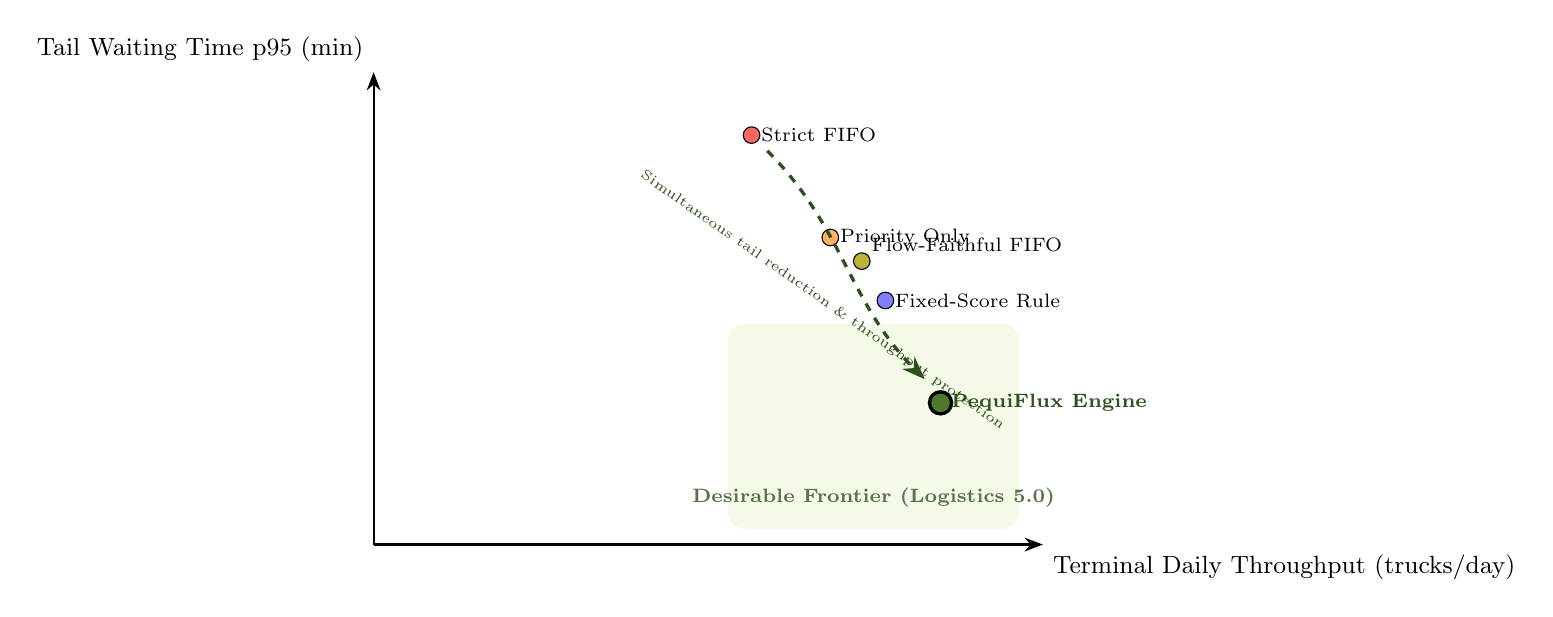
\begin{tikzpicture}[>=Stealth, font=\small]
  \draw[->, thick] (0,0) -- (8.5,0) node[below right] {Terminal Daily Throughput (trucks/day)};
  \draw[->, thick] (0,0) -- (0,6.0) node[above left] {Tail Waiting Time p95 (min)};

  % Desirable quadrant shading
  \fill[pequiLight!60, rounded corners=6pt] (4.5,0.2) rectangle (8.2,2.8);
  \node[font=\scriptsize\bfseries, text=pequiDark!80] at (6.35,0.6) {Desirable Frontier (Logistics 5.0)};

  % Points
  \filldraw[fill=red!60, draw=black] (4.8,5.2) circle (3pt) node[right, font=\scriptsize] {Strict FIFO};
  \filldraw[fill=orange!60, draw=black] (5.8,3.9) circle (3pt) node[right, font=\scriptsize] {Priority Only};
  \filldraw[fill=yellow!70!black, draw=black] (6.2,3.6) circle (3pt) node[above right, font=\scriptsize] {Flow-Faithful FIFO};
  \filldraw[fill=blue!50, draw=black] (6.5,3.1) circle (3pt) node[right, font=\scriptsize] {Fixed-Score Rule};
  \filldraw[fill=pequiLeaf, draw=black, very thick] (7.2,1.8) circle (4pt) node[right, font=\scriptsize\bfseries, text=pequiDark] {PequiFlux Engine};

  % Trajectory arrow
  \draw[->, very thick, dashed, draw=pequiDark] (5.0,5.0) to[out=-45,in=135] (7.0,2.1);
  \node[font=\tiny, text=pequiDark, rotate=-35] at (5.7,3.1) {Simultaneous tail reduction \& throughput protection};
\end{tikzpicture}%
}
\caption{Operational trade-off frontier between daily terminal throughput and tail waiting time (p95).}
\label{fig:tradeoff}
\end{figure}

\subsection{Resilience to Stochastic Operational Disruptions}
The experimental results demonstrate remarkable resilience under the \emph{Weather} and \emph{Compound} disruption regimes. When rainfall forces the closure of open hoppers, Strict FIFO induces cascading paralysis: trucks assigned to open hoppers wait at the head of the buffer queue, blocking subsequent covered-hopper trucks from reaching initial weighing. 

In contrast, the PequiFlux engine instantly updates $C_{k,r}$, removing weather-sensitive assignments while allowing trucks destined for covered hoppers to advance through shared scale pool $B$. Once rain ceases, the dynamic operational pressure term $\hat{P}_i(k)$ prioritizes the accumulated backlog of delayed trucks, smoothing the recovery wave without causing internal gridlock.

\subsection{Safety Verification (A1) and Governance Auditability (A2)}
Across all 18,000 policy-day simulations, the automated assertion verification confirmed:
\begin{itemize}[leftmargin=1.2cm,itemsep=0pt,topsep=2pt]
  \item \textbf{A1 Pass Rate: 100\% (0 violations)}. No truck was dispatched to an incompatible hopper, weighed out of sequence, or routed to an unverified quality status.
  \item \textbf{A2 Traceability: 100\% structural completeness}. All decisions generated valid JSONL logs recording timestamps, resource identifiers, admissible candidate sets, and human-readable sorting rationales. In trials featuring synthetic supervisor overrides, valid operator adjustments were seamlessly accommodated while invalid override attempts (e.g., forcing an uninspected truck to unload) were safely rejected and logged with cause.
\end{itemize}

\subsection{Managerial Implications for Production and Logistics Engineering}
These findings offer practical guidelines for operations managers and terminal designers:
\begin{enumerate}[leftmargin=1.2cm,itemsep=0pt,topsep=2pt]
  \item \textbf{Decoupling Reentrant Contention}: Shared weighbridges represent a systemic vulnerability. Managing them through dynamic online dispatching rather than segregated FIFO lanes unlocks up to 18\% additional throughput during harvest spikes without physical civil expansion.
  \item \textbf{Human-in-the-Loop Operations}: Black-box optimization often engenders operator distrust. By providing explicit lexicographic explanations and retaining supervisory veto power, the proposed artifact fosters operator acceptance and supports continuous process improvement.
  \item \textbf{Digital Models as Risk-Free Proving Grounds}: Coupling DES engines with 3D digital models enables facility managers to rehearse harvest arrival surges, test layout modifications, and train operators prior to actual harvest deployment.
\end{enumerate}

% =========================================================================
\section{Conclusions and Future Work}
\label{sec:conclusion}
% =========================================================================

This research modeled, implemented, and evaluated an online constrained dispatching decision-support engine for agro-industrial receiving yards, framed within the principles of Logistics 5.0. By modeling the yard as a Dynamic Reentrant Hybrid Flow Shop with shared scales, the proposed artifact resolves the critical tension between operational throughput, strict physical constraints, and unpredictable environmental disruptions.

Computational experiments spanning 72 factorial configurations and 18,000 policy runs confirmed hypothesis H1: the engine achieves a greater than $15\%$ reduction in p95 queue waiting time across medium and high congestion strata without compromising throughput. Concurrently, criteria A1 and A2 ensure absolute operational safety and transparent, auditable governance.

\subsection{Limitations and Future Research Directions}
Several promising avenues remain for extending this work:
\begin{enumerate}[leftmargin=1.2cm,itemsep=0pt,topsep=2pt]
  \item \textbf{Mathematical Programming Bounds (MILP)}: Formulating an offline rolling-horizon Mixed-Integer Linear Program with perfect information would provide an exact theoretical upper bound to quantify the absolute optimality gap of the online heuristic.
  \item \textbf{Deep Reinforcement Learning (RL)}: Extending the decision logic to a Markov Decision Process (MDP) with Action Masking could enable the discovery of adaptive dispatching policies that anticipate future arrival cascades.
  \item \textbf{Bi-Objective Green Logistics}: Incorporating vehicle idling fuel consumption and greenhouse gas ($\text{CO}_2$, $\text{NO}_x$) emission factors would allow multi-objective Pareto optimization, directly aligning terminal operations with industrial sustainability targets.
  \item \textbf{Bidirectional Digital Twin Integration}: Expanding the Unreal Engine 5.8 digital model with real-time IoT RFID sensing and automated gate actuation will bridge the gap toward a fully synchronized digital twin.
\end{enumerate}

\section*{Acknowledgements}
The authors acknowledge the Pontifical Catholic University of Goi{\'a}s (PUC Goi{\'a}s) for academic infrastructure and support.

\printbibliography

\end{document}
